\section{P-I-D analysis}\label{p-i-d-analysis}

This report introduces the effects of proportional, derivative and
integral terms for a typical PID controller. The effect of varying gain
is assessed using time-domain and root locus results. For a closed loop
classical PID controller, the basic aim is to reduce tracking error
between the control input and the observed output. In an engineering
context, it is desirable to have a sharp response to user input and
correctly tuned PIDs will achieve this. The responses highlighted in
this report are in relation to the Quanser behaviour observed in Control
Coursework Part 1.

\subsection{Proportional Feedback
Controller}\label{proportional-feedback-controller}

\begin{wrapfigure}{l}{0.5\textwidth}
\centering
\vspace{-15pt} % Space added to the top of the image
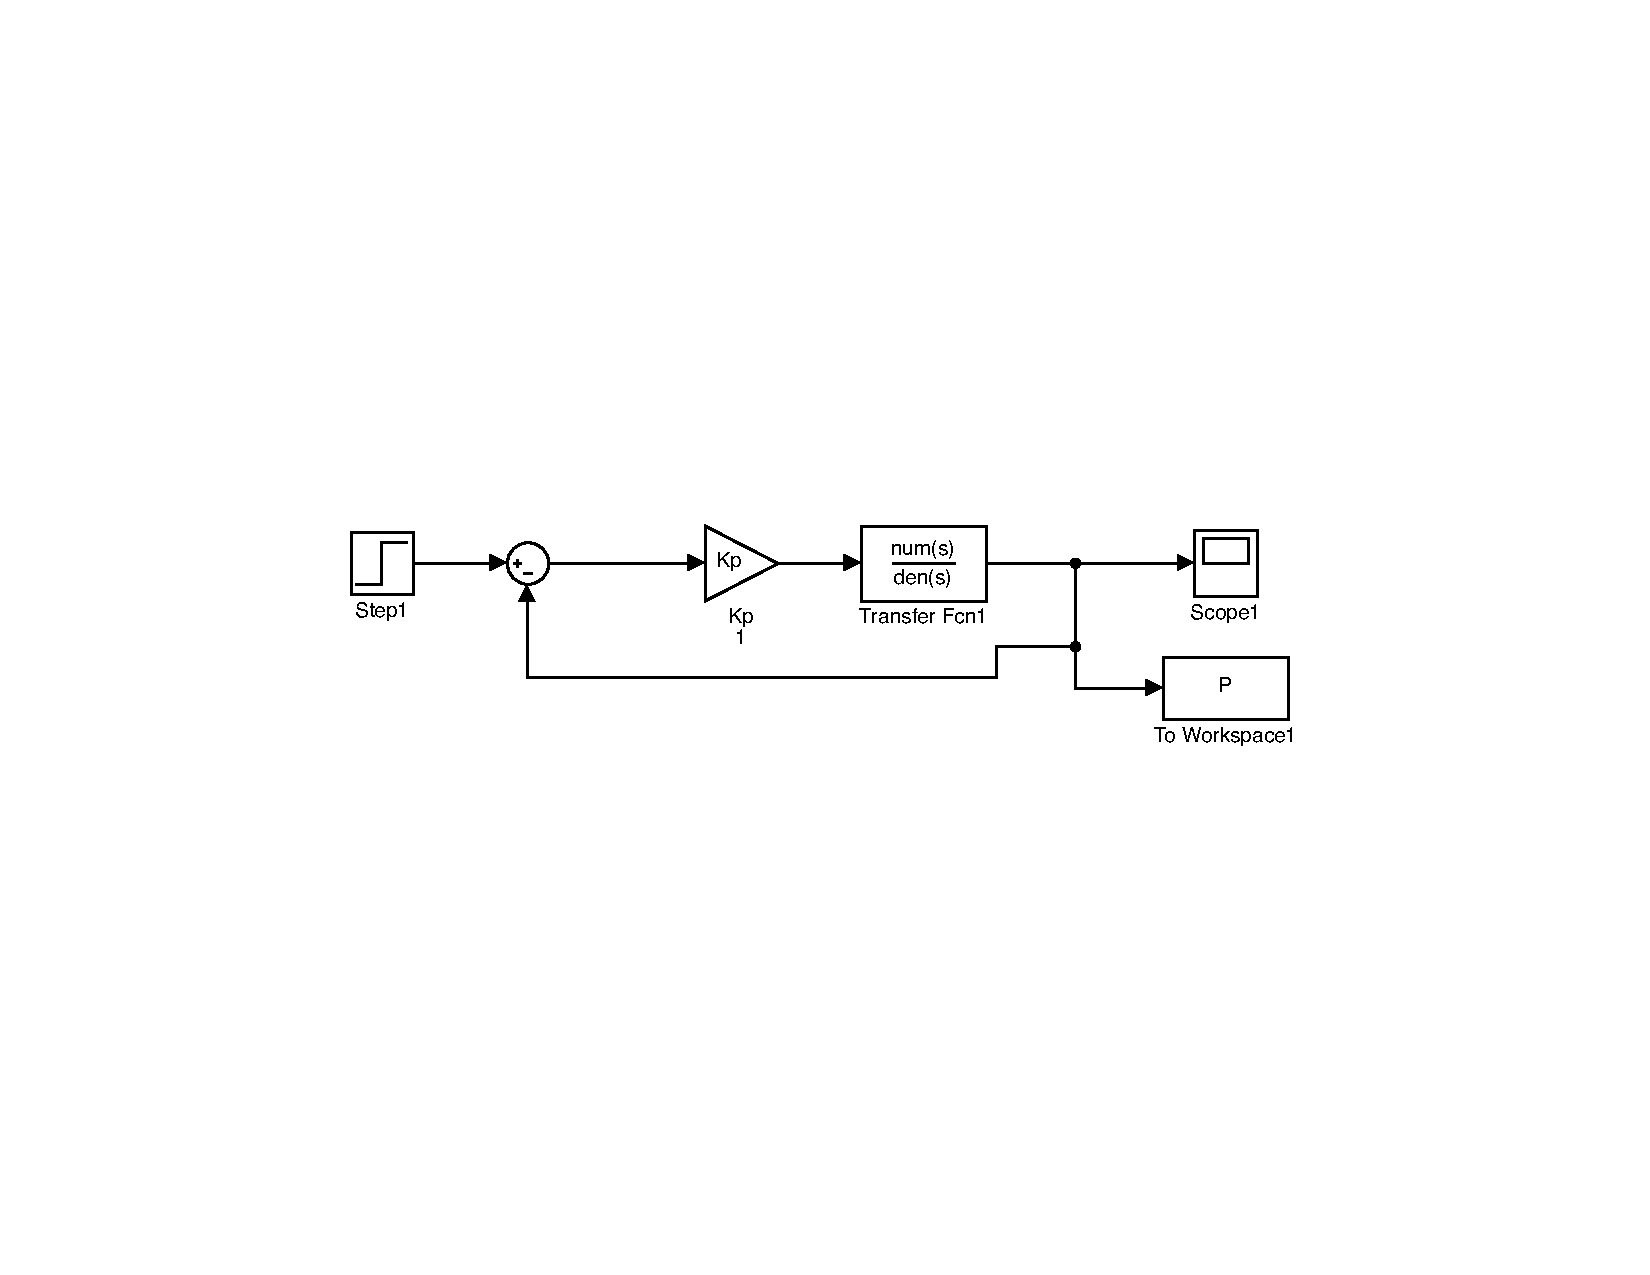
\includegraphics[trim = 0 0 0 0, clip, width=0.5\textwidth]{Psim.pdf}
\vspace{-10pt}
\caption{Caption Text}
\label{Psim}
\vspace{-15pt}
\end{wrapfigure}

Proportional control uses the `Present' state of the plant to error
correct. The correction applied is proportional to the deviation from
the desired state of the plant. This implies a highly oscillatory system
response, as the present error doesn't take into account the past or
future but rather the instantaneous state of the plant. The effect of
varying proportional gain (Kp) was observed through the simulation built
in REFERENCE. This simulation was executed in an iterative loop with
varying Kp from 0 to 0.1 in increments of 0.01. REFERENCE shows the time
domain response of increasing Kp. When Kp = 0, a flat line is observed
as there is no signal passing through the plant. With increasing
proportional gain, the correction factor becomes larger and as seen by
the increased amplitude for higher Kp gains. The `stepinfo()' function
shows that increasing Kp -- reduces rise time and steady state error
whilst increasing overshoot.

The root locus plot in REFERENCE allows observation of s-domain features
with varying proportional gain. For pure variation in proportional gain,
the (stable) poles are restricted to the same distance from the
imaginary axis. In addition, increasing Kp moves the poles away from the
real axis in both directions. This implies increased natural frequency
with increased Kp and decreased damping ratio. This verifies the
observation noted in the time domain plot, as increased natural
frequency will lead to greater oscillatory behaviour and decreased
damping ratio increases the overshoot.

\begin{figure}[H]
\centering
\begin{minipage}{.455\textwidth}
 \centering
 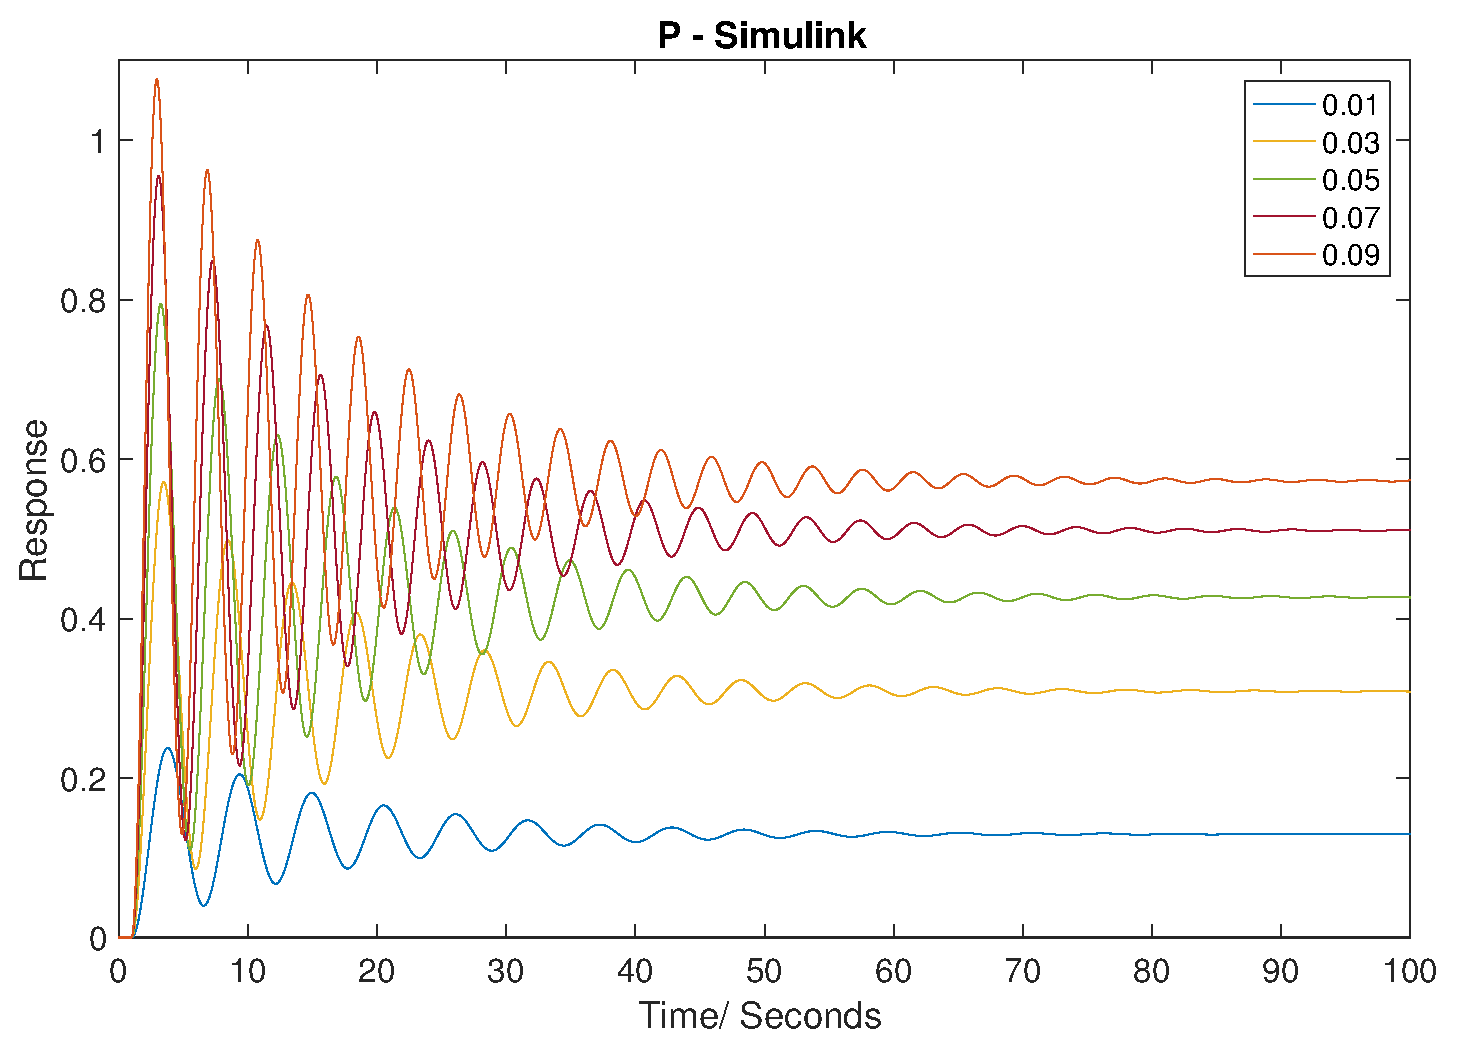
\includegraphics[trim = 0 0 0 0, clip, width=1\textwidth]{pres.eps}
 \caption{}
 \label{pres}
\end{minipage}
\hfill
\begin{minipage}{.455\textwidth}
\centering
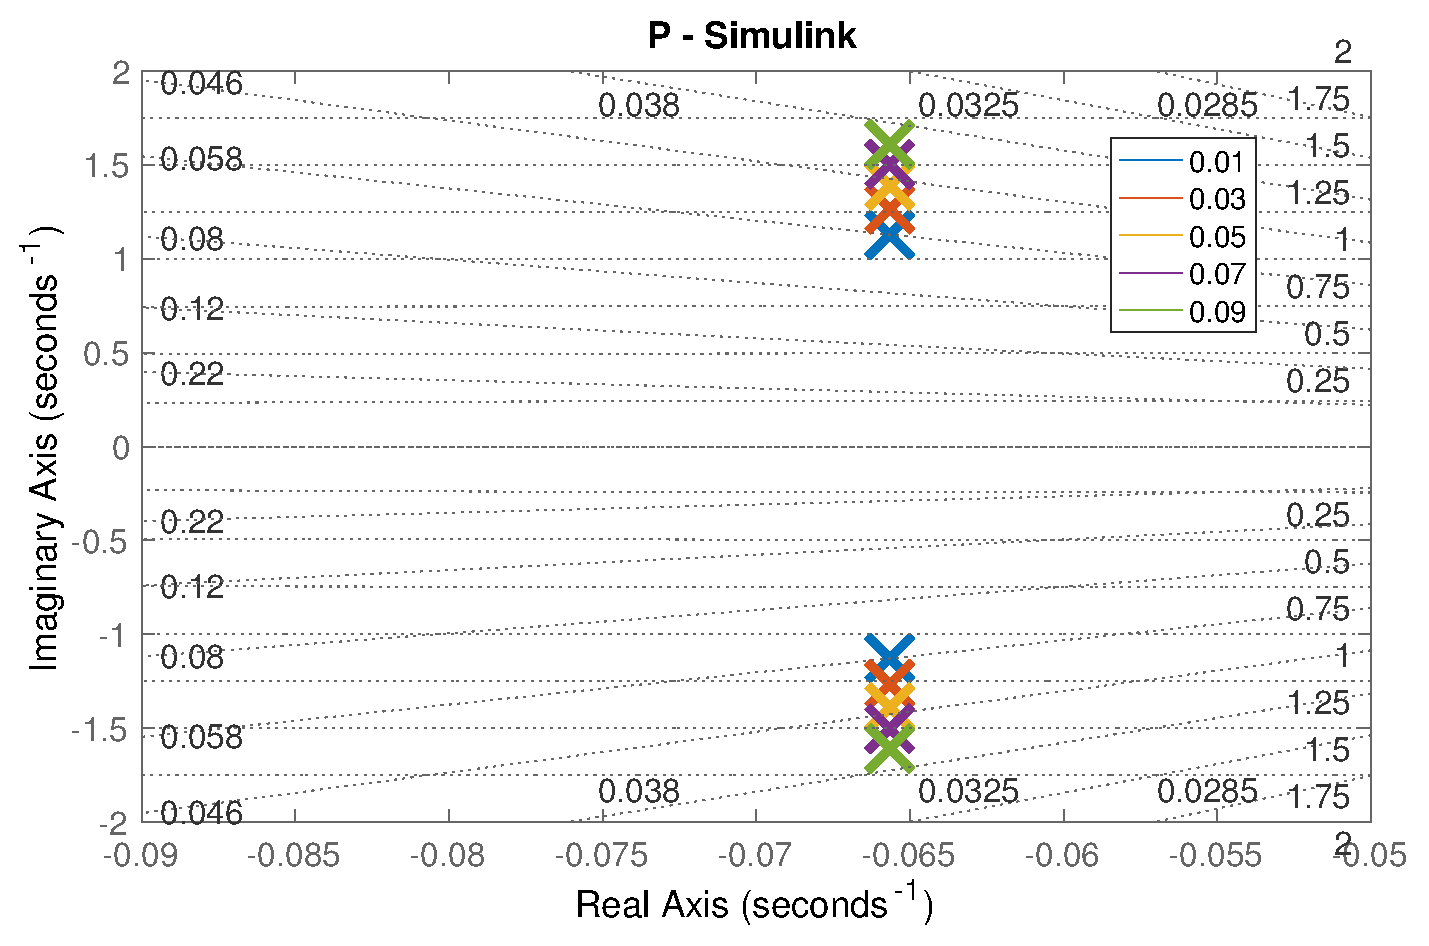
\includegraphics[trim = 0 0 0 0, clip, width=1\textwidth]{pzp.eps}
\caption{}
\label{pzp}
\end{minipage}
\vspace{-20pt}
\end{figure}

\subsection{Derivative Feedback
Controller}\label{derivative-feedback-controller}

\begin{wrapfigure}{l}{0.5\textwidth}
\centering
\vspace{-15pt} % Space added to the top of the image
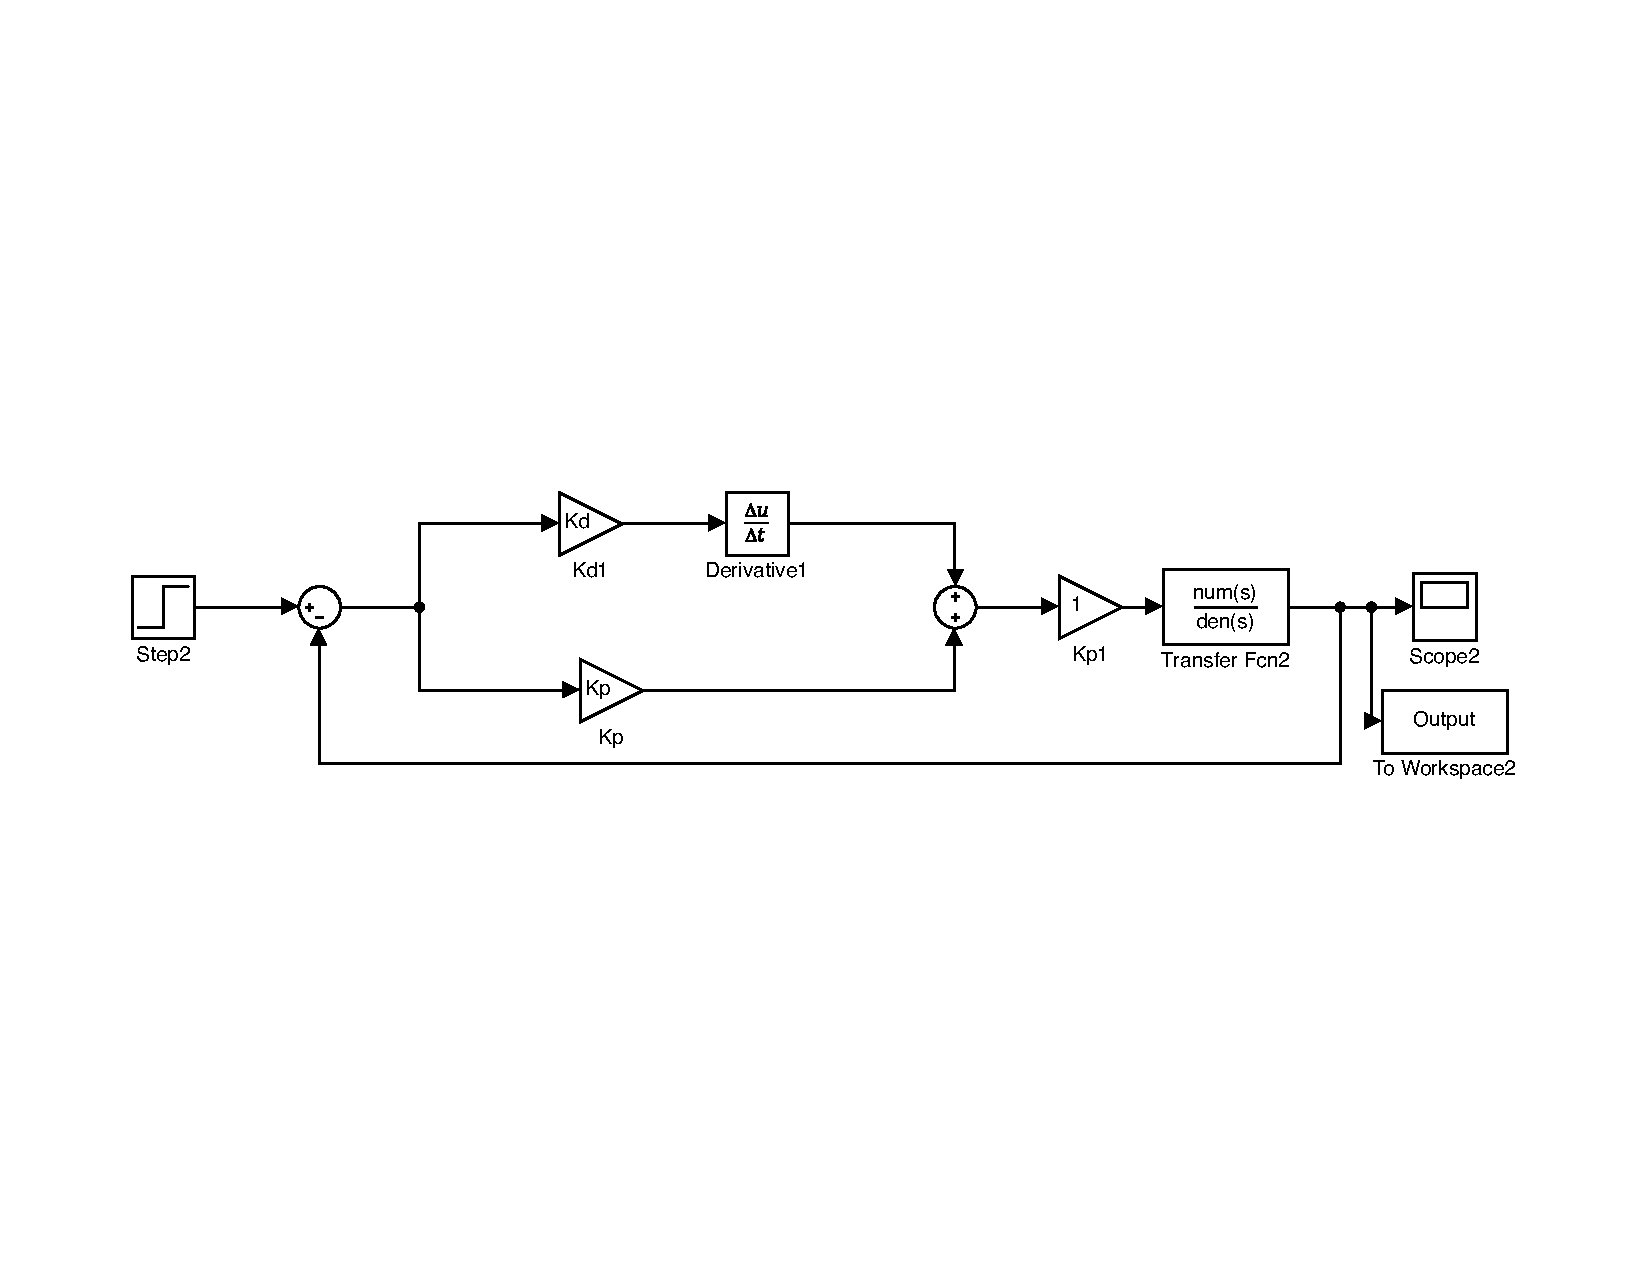
\includegraphics[trim = 0 0 0 0, clip, width=0.5\textwidth]{pd2.pdf}
\vspace{-10pt}
\caption{Caption Text}
\label{pd2}
\vspace{-15pt}
\end{wrapfigure}

Derivative control utilises the expected `Future' state of the system to
pre-emptively produce an error correct signal. This correction is
proportional to the rate of change of the system state at a point in
time. The system calculates the state of the plant in the future based
on rate of change conditions correctly and accounts for that by
anticipating the response. For this reason a large damping effect is
expected for increasing derivative gain (Kd). The simulation in
REFERENCE was implemented to observe two things -- first the effect of
purely varying derivative gain with constant proportional gain, and
second the effect of varying both gains by the same amount -- this was
controlled using the additional gain block after the controller. The
gain/s in both REFERENCE and REFERENCE was incremented from 0 to 1 in
increments of 0.05.

As expected, the time domain responses show that increasing Kd has a
greater damping effect on oscillations. There is a reduction in
overshoot and increase in rise time. For a Kd = 0 , large oscillations
are observed and decrease with increasing gain. For larger gain values
of 0.6 and above there is high damping with the response settling to a
steady level quickly. Increasing both Kd and Kp by the same amount shows
reduction in rise time, overshoot and steady state error. PD control
appears more effective.

The root locus S-domain metrics show that as Kd is increased the poles
are shifted more negatively in the real axis. The semi-circular shape
represents the line of equal proportional gain and points represent
varying Kd at that Kp level. As Kd increases the angle between the
imaginary axis increases -- this implies poles closer to the real axis,
ie higher Kd corresponding poles have greater damping; natural frequency
is reduced (and hence less oscillatory behaviour).

\subsection{Integral Action}\label{integral-action}

\begin{wrapfigure}{l}{0.5\textwidth}
\centering
\vspace{-15pt} % Space added to the top of the image
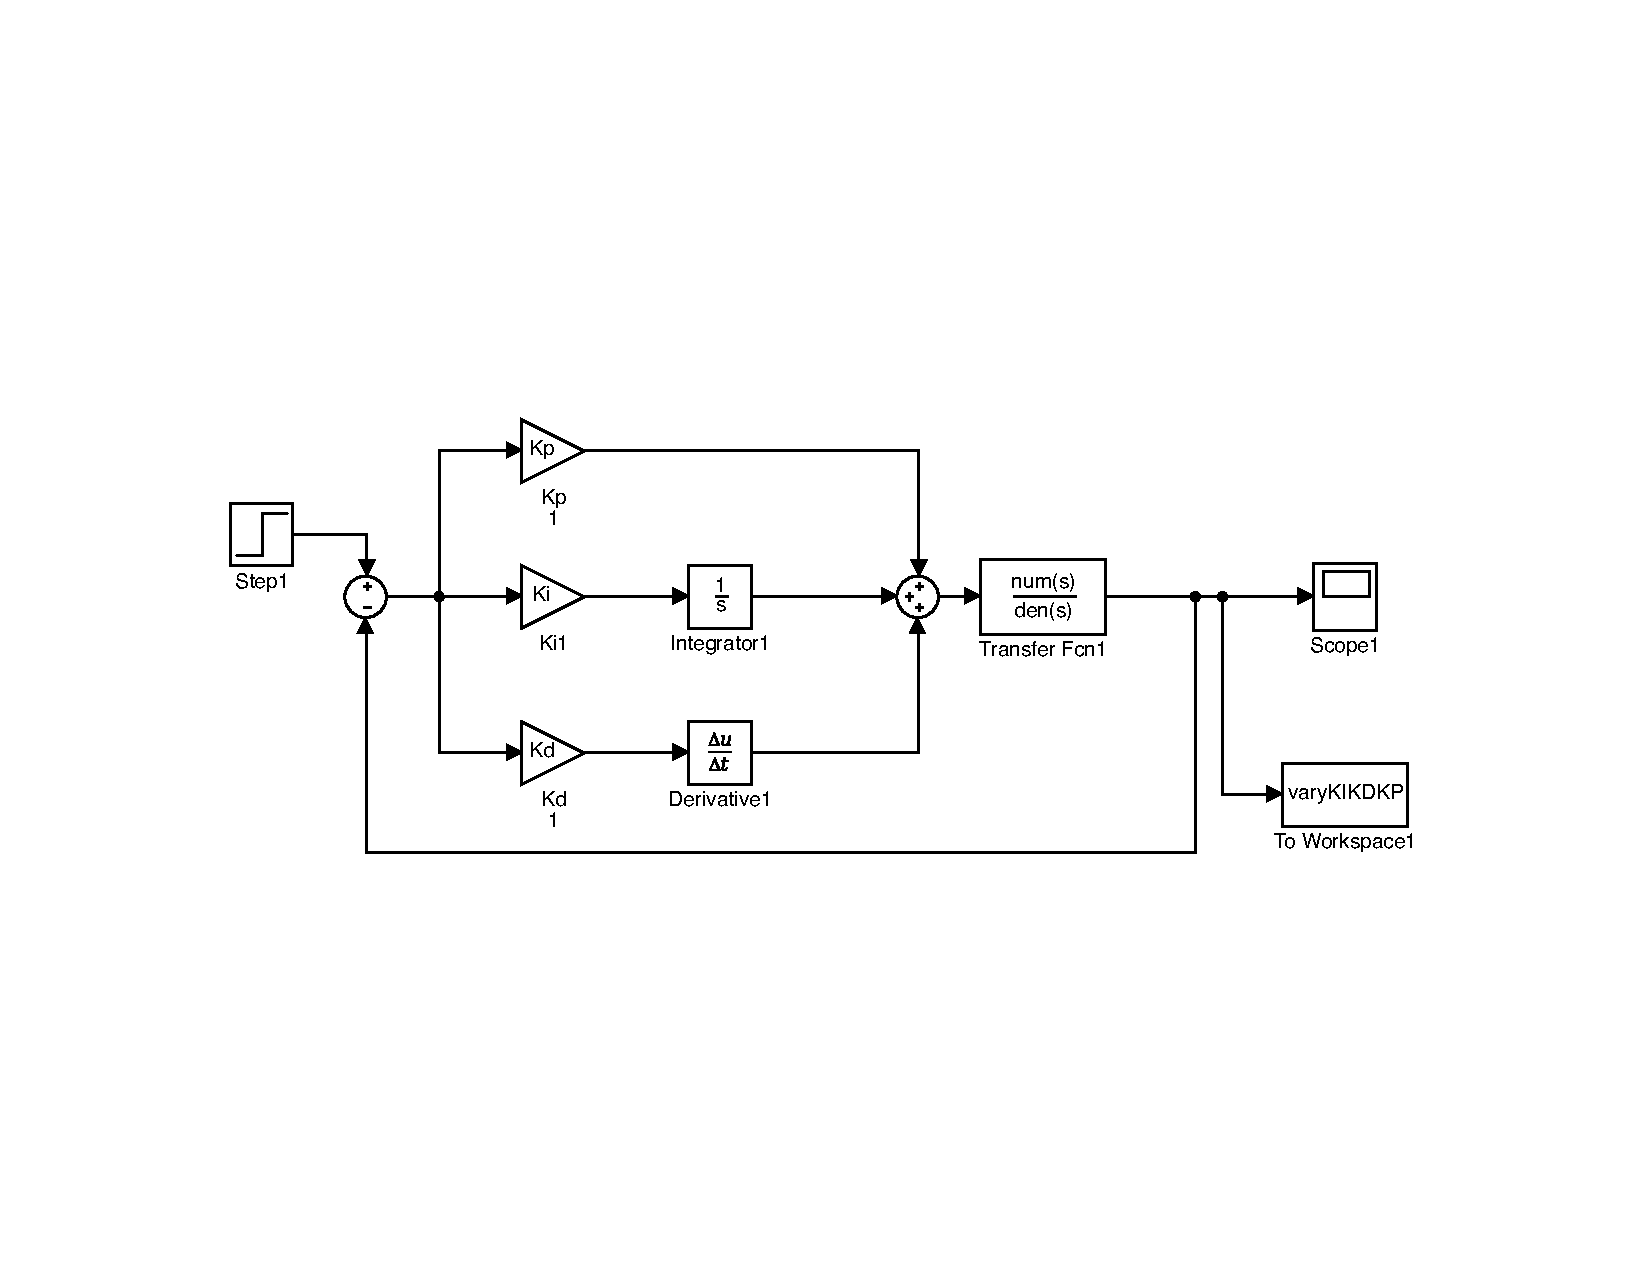
\includegraphics[trim = 0 0 0 0, clip, width=0.5\textwidth]{PIDp2.pdf}
\vspace{-10pt}
\caption{Caption Text}
\label{PIDp2}
\vspace{-15pt}
\end{wrapfigure}

Integral control utilises the `Past' state of the system to produce an
error-correcting signal. The integral term looks at the period and how
far the measured variable is from the desired state in time. This
controller sums the complete error in history up to current time state.
For this reason the integral control will eliminates offset and leads to
zero steady state error. REFERENCE shows the variation of pure Ki with
constant Kp and Kd. REFERENCE shows the variation of all three gains Kd,
Ki and Kp by the same magnitude -- this was implemented using a
gain-scaling block after the controller. The time domain plots confirm
the zero steady state error as the oscillations level to desired
response level.

0 there is steady state error that exists in the system, but as integral
gain increases the steady state error is completely eliminated. The
preferred controller is PID.

\section{PID Design to Achieve Control
Requirements}\label{pid-design-to-achieve-control-requirements}

\subsection{Open Loop Transfer Function PID
Controller}\label{open-loop-transfer-function-pid-controller}

\subsection{Tuned Quanser Controller}\label{tuned-quanser-controller}
